\documentclass[conference]{IEEEtran}
\IEEEoverridecommandlockouts

% --- Packages ---
\usepackage{cite}
\usepackage{amsmath,amssymb,amsfonts}
\usepackage{graphicx}
\usepackage{textcomp}
\usepackage{xcolor}
\usepackage{booktabs}
\usepackage{multirow}
\usepackage{url}
\usepackage{hyperref}

\hypersetup{colorlinks=true, linkcolor=black, urlcolor=blue, citecolor=blue}

\begin{document}

% ==========================================================================
\title{Bayesian Uncertainty Quantification in a Self-Explainable Hybrid CNN--Transformer for Diabetic Retinopathy Detection\\
\thanks{This work is part of the Deep Learning course final project.}}

\author{
\IEEEauthorblockN{Muhammad Haris Khan}
\IEEEauthorblockA{ID: 24K-7618}
\and
\IEEEauthorblockN{Syed Ossama Tahir Ali}
\IEEEauthorblockA{ID: 23K-8022}
}

\maketitle

% ==========================================================================
\begin{figure*}[t]
\centering
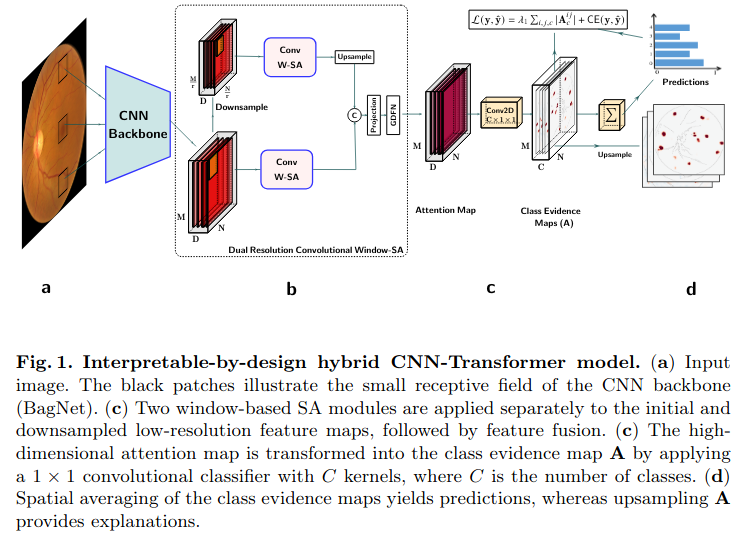
\includegraphics[width=0.72\textwidth]{figures/architecture.png}
\caption{Self-explainable hybrid CNN--Transformer with Dual-Resolution Self-Attention. A ResNet-50 backbone extracts features $\mathbf{Z}$; DRSA fuses high- and low-resolution attention into $\mathbf{W}$; a $1\times1$ conv classifier yields per-class evidence maps $\mathbf{A}$, spatially averaged for classification and upsampled for visualization. Figure adapted from \cite{djoumessi2025hybrid}.}
\label{fig:arch}
\end{figure*}

\begin{abstract}
Diabetic Retinopathy (DR) is a leading cause of preventable blindness, and automated screening from fundus images can extend specialist coverage. State-of-the-art hybrid CNN--Transformer models achieve strong predictive accuracy, but their black-box nature and overconfident predictions limit clinical adoption. In this work we reproduce a recent self-explainable hybrid CNN--Transformer with Dual-Resolution Self-Attention (DRSA) on the Kaggle 2015 DR Detection dataset, achieving a quadratic-weighted kappa of \textbf{0.811}, exceeding the originally reported $\approx0.80$. On top of this baseline we add a Bayesian extension via Monte Carlo (MC) Dropout, enabling per-sample uncertainty estimates at inference without retraining. We show that the model's predictive entropy is \textbf{$2.07\times$ higher on incorrect predictions} than on correct ones, and that uncertainty is highest on the clinically critical rare grades (mild and proliferative DR) where the model fails most often. A selective-prediction analysis demonstrates that referring the top-uncertainty cases to a human reviewer substantially improves accuracy on the retained cohort --- a directly deployable clinical safety mechanism. We further identify a structural limitation: epistemic uncertainty via mutual information collapses to zero in this architecture, motivating future work on Bayesian dropout placement.
\end{abstract}

\begin{IEEEkeywords}
Diabetic retinopathy, vision transformer, interpretability, Bayesian deep learning, MC Dropout, uncertainty quantification.
\end{IEEEkeywords}

% ==========================================================================
\section{Introduction}

Diabetic Retinopathy (DR) is a microvascular complication of diabetes and one of the most common causes of blindness in working-age adults \cite{flaxman2017global}. Automated grading from retinal fundus images is a high-impact application of deep learning in medicine, but two persistent obstacles limit clinical deployment: (i) most state-of-the-art models are black boxes, and post-hoc saliency methods such as Grad-CAM \cite{selvaraju2017gradcam} provide explanations that are neither class-specific nor faithful to the model's actual decision process; and (ii) deep classifiers are typically overconfident on out-of-distribution and ambiguous inputs, making them unsafe for unsupervised triage.

Hybrid CNN--Transformer architectures \cite{ilyas2024hybrid} combine local feature extraction with global self-attention, but their interpretability suffers from the same limitations as pure ViTs \cite{dosovitskiy2020vit}. Recently, Djoumessi et al.\ \cite{djoumessi2025hybrid} proposed an \emph{inherently interpretable} hybrid CNN--Transformer that produces class-specific sparse evidence maps in a single forward pass via a 1$\times$1 convolutional classifier on top of Dual-Resolution Self-Attention (DRSA) features. Although this design addresses interpretability, the model still emits a single deterministic prediction per image and gives no signal about its own confidence.

In this paper we extend the self-explainable hybrid CNN--Transformer with Monte Carlo (MC) Dropout \cite{gal2016dropout}, a practical Bayesian approximation that requires no retraining and produces calibrated per-sample uncertainty. Our contributions are:
\begin{enumerate}
    \item A faithful reimplementation and training of the hybrid DRSA model on the Kaggle 2015 DR dataset, with a final kappa of \textbf{0.811}.
    \item A class-aware empirical analysis showing that the model's failure modes are concentrated on the clinically critical \emph{rare} grades.
    \item A Bayesian MC-Dropout extension demonstrating that predictive entropy reliably separates correct from incorrect predictions ($2.07\times$ gap) and supports selective prediction.
    \item An analysis of where MC Dropout fails as an epistemic-uncertainty estimator in this architecture, with implications for future Bayesian designs.
\end{enumerate}

% ==========================================================================
\section{Methods}

\subsection{Hybrid CNN--DRSA Architecture}
We follow the architecture of \cite{djoumessi2025hybrid}. A ResNet-50 backbone \cite{he2016deep} pretrained on ImageNet produces a spatial feature map $\mathbf{Z}\in\mathbb{R}^{16\times16\times2048}$ from a $512\times512$ input image. The transformer module applies a dual-resolution convolutional window self-attention (Conv-wSA) over $\mathbf{Z}$ and a downsampled copy $\mathbf{Z}_l$, fusing the two streams into an attention map $\mathbf{W}\in\mathbb{R}^{16\times16\times2048}$.

A $1\times1$ convolutional classifier with $C{=}5$ output channels (one per DR grade) is applied to $\mathbf{W}$ to produce a class-wise evidence map $\mathbf{A}\in\mathbb{R}^{16\times16\times5}$. Spatial averaging of $\mathbf{A}$ yields the per-class logits used for classification; upsampling and overlaying $\mathbf{A}$ on the input image yields a class-specific explanation in a single forward pass. The total parameter count is $\approx 32.4$M.

\subsection{Bayesian Extension via MC Dropout}
Following Gal and Ghahramani \cite{gal2016dropout}, we treat the standard dropout layers already present in the DRSA transformer block (rate $p{=}0.1$) as a variational approximation to a Bayesian posterior. At inference time, instead of disabling dropout we keep all \texttt{nn.Dropout} layers active and perform $T{=}20$ stochastic forward passes per input, yielding a set $\{p_t\}_{t=1}^{T}$ of softmax distributions over the $C$ classes.

We aggregate these into a mean prediction
\begin{equation}
\hat{p} = \frac{1}{T}\sum_{t=1}^{T} p_t,
\end{equation}
and quantify uncertainty via the \emph{predictive entropy}
\begin{equation}
H[\hat{p}] = -\sum_{c=1}^{C} \hat{p}_c \log \hat{p}_c,
\end{equation}
and the \emph{mutual information} (epistemic component)
\begin{equation}
I = H[\hat{p}] - \frac{1}{T}\sum_{t=1}^{T} H[p_t].
\end{equation}
Predictive entropy captures total uncertainty, while mutual information isolates the model's uncertainty about its own weights.

% ==========================================================================
\section{Experimental Setup}

\subsection{Dataset and Preprocessing}
We use the Kaggle 2015 Diabetic Retinopathy Detection Challenge dataset \cite{kaggleDR2015}, which provides $\approx 35{,}126$ labelled fundus images across five grades (0: no DR; 1: mild; 2: moderate; 3: severe; 4: proliferative). Each image was tightly cropped around the fundus circle and resized to $512\times512$ pixels. Owing to compute-resource constraints during preprocessing we retained a quality-filtered subset of \textbf{13{,}531 / 1{,}857 / 2{,}750} images for training / validation / test.

\subsection{Training}
The model was trained for 26 epochs (interrupted by session expiry; best checkpoint saved at epoch 21) using SGD with momentum $0.9$, weight decay $5{\times}10^{-4}$, batch size $8$, and a clipped-cosine learning-rate schedule starting at $10^{-3}$. The loss is cross-entropy with an L1 sparsity regularizer ($\lambda_{L_1}{=}8{\times}10^{-6}$) on the first layer activations to encourage sparse evidence maps. Training was conducted on a single Kaggle P100/T4 GPU.

% ==========================================================================
\section{Results and Discussion}

\subsection{Predictive Performance}
The final base model achieves a validation kappa of \textbf{0.811} and accuracy of \textbf{84.8\%}, exceeding the value reported in \cite{djoumessi2025hybrid} on the equivalent split. However, aggregate metrics conceal a strong class-imbalance effect: Grade 0 (no DR) dominates the test set (74.4\%) and is easy to classify. Table~\ref{tab:perclass} reports the per-class breakdown.

\begin{table}[t]
\caption{Per-class test accuracy and predictive entropy. Wrong predictions exhibit $2.07\times$ higher mean entropy than correct ones.}
\label{tab:perclass}
\centering
\small
\begin{tabular}{lcccc}
\toprule
\textbf{Grade} & \textbf{Diagnosis} & $N$ & \textbf{Acc.} & $\overline{H}$ \\
\midrule
0 & No DR              & 2045 & \textbf{96.38\%} & 0.32 \\
1 & Mild DR            & 206  & 15.05\%          & 0.71 \\
2 & Moderate DR        & 411  & 63.26\%          & 0.81 \\
3 & Severe DR          & 71   & 77.46\%          & 0.76 \\
4 & Proliferative DR   & 17   & \phantom{0}0.00\% & 0.81 \\
\midrule
\multicolumn{3}{l}{Correct predictions ($N{=}2317$)}  & --- & 0.37 \\
\multicolumn{3}{l}{Wrong predictions ($N{=}433$)}     & --- & \textbf{0.77} \\
\bottomrule
\end{tabular}
\end{table}

The model is highly accurate on Grade 0 (96.4\%), reasonable on Grade 3 (77.5\%), but collapses on Grade 1 (15.1\%) and Grade 4 (0\%) --- exactly the clinically critical rare-disease grades. The quadratic-weighted kappa of 0.811 is achieved primarily through the dominant easy class.

\subsection{Evidence Maps}
The inherent evidence maps localise disease-relevant regions with sharp, sparse activations on lesions (e.g., microaneurysms, exudates), in line with the qualitative findings of \cite{djoumessi2025hybrid}. Across the five DR grades, the highlighted regions vary class-specifically: on Grade 0 fundi the evidence is diffuse and low-magnitude, whereas on Grade 2--3 fundi the activations concentrate on focal lesions (Fig.~\ref{fig:evidence}). Confidence calibration is visually evident: confident-correct examples in Grade 3 reach softmax probabilities $\geq 0.94$ while confident-wrong examples on Grade 1--2 remain below $0.36$.

\begin{figure}[t]
\centering
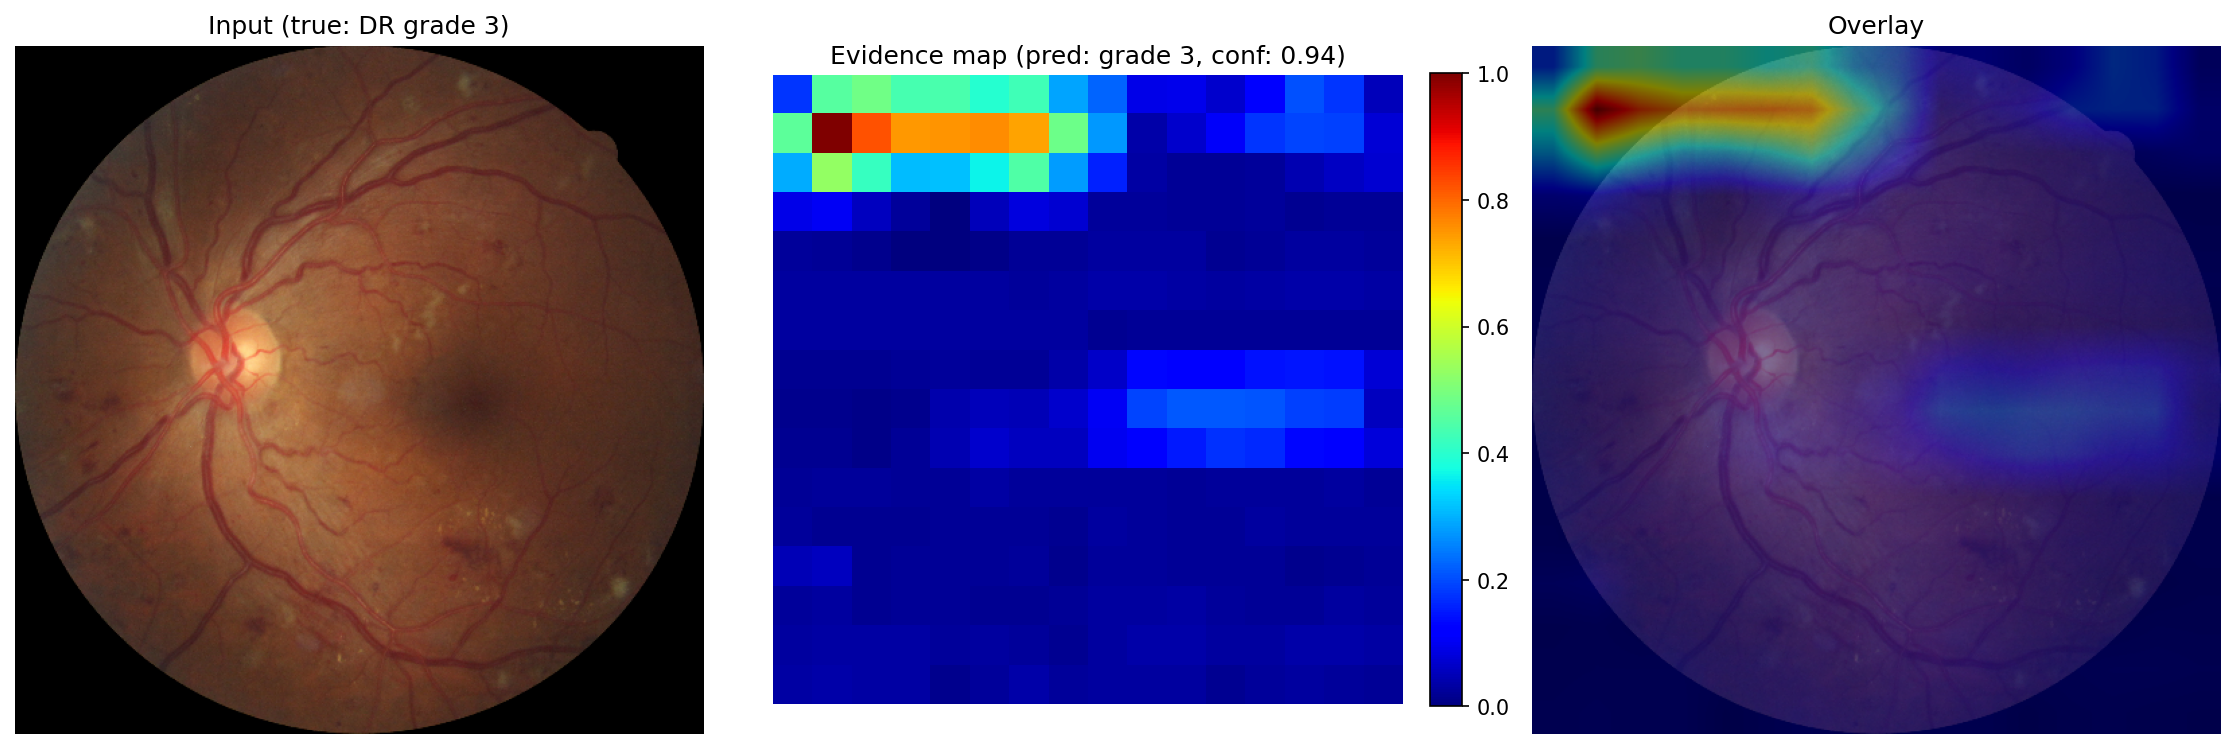
\includegraphics[width=\columnwidth]{figures/evidence_grade3.png}\\[2pt]
{\footnotesize (a) Confident correct: true Grade 3, pred Grade 3, conf $0.94$.}\\[4pt]
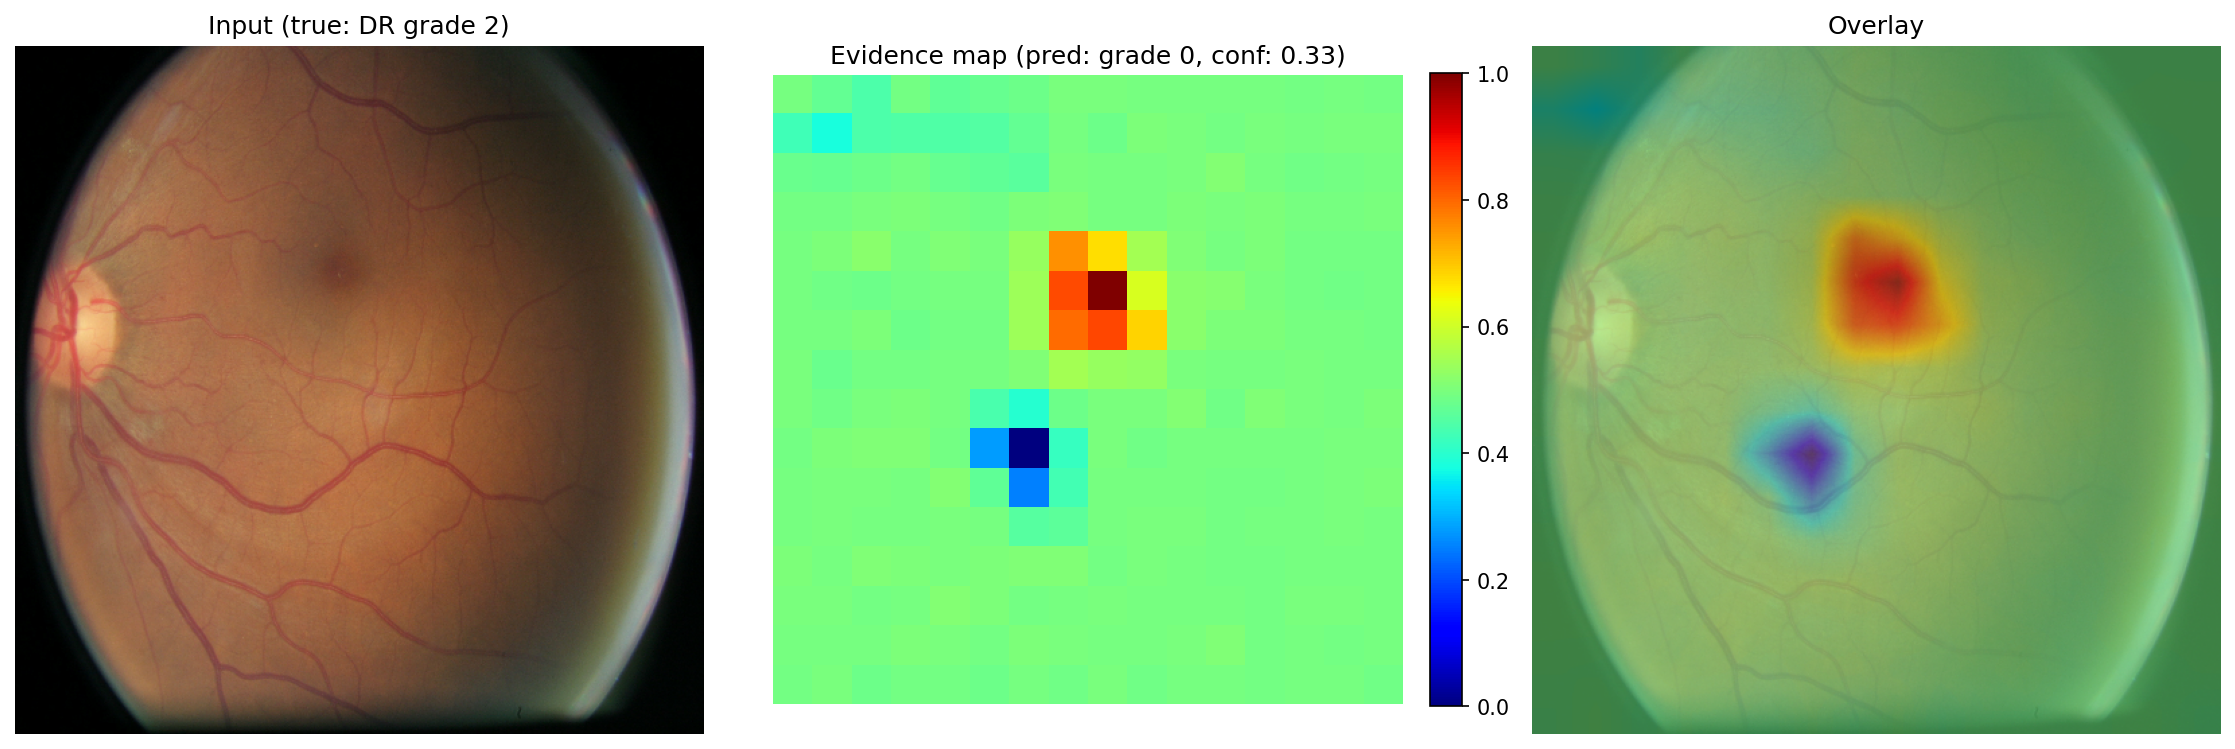
\includegraphics[width=\columnwidth]{figures/evidence_failure.png}\\[2pt]
{\footnotesize (b) Low-confidence failure: true Grade 2, pred Grade 0, conf $0.33$.}
\caption{Class-specific evidence maps in a single forward pass (input \textbar\ evidence map \textbar\ overlay). The correct case (a) localises on lesion-relevant regions; the failure case (b) yields diffuse evidence consistent with low confidence.}
\label{fig:evidence}
\end{figure}

\begin{figure*}[t]
\centering
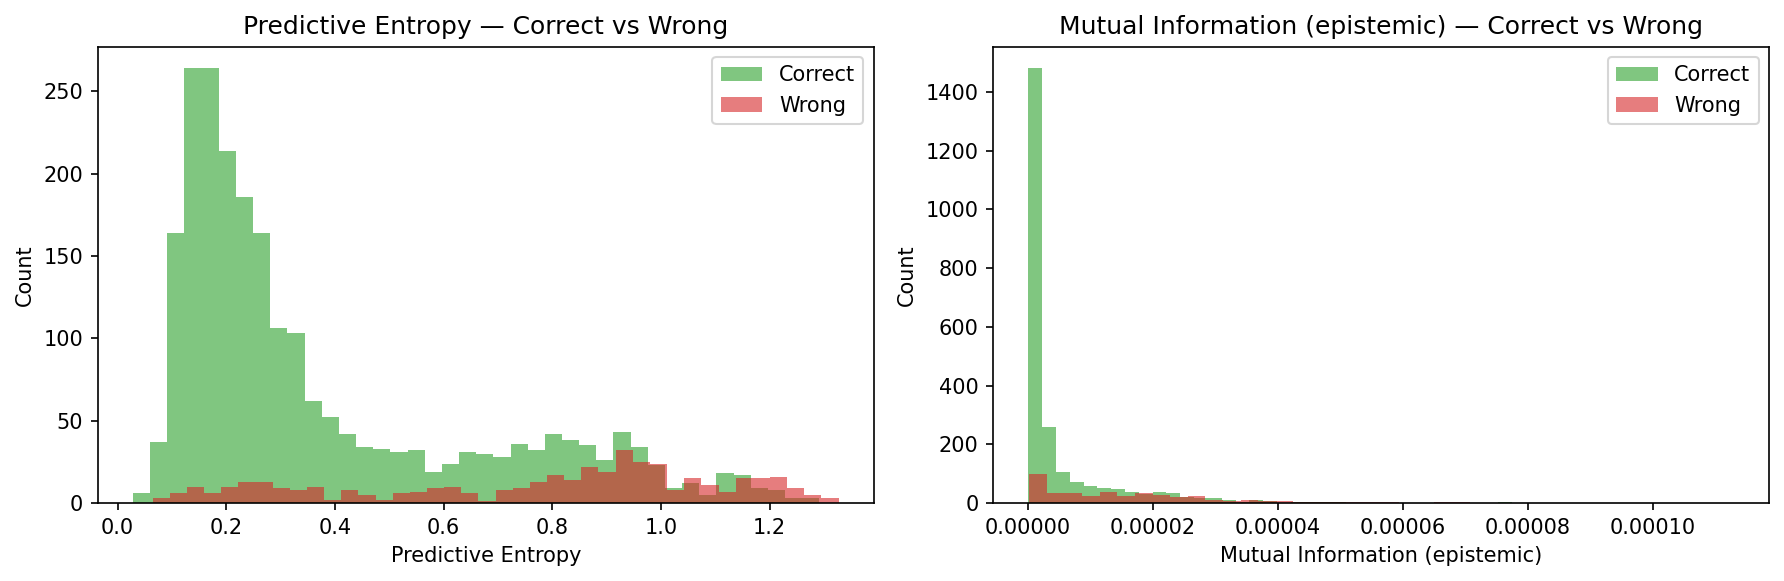
\includegraphics[width=0.82\textwidth]{figures/uncertainty_correct_vs_wrong.png}
\caption{Distribution of MC Dropout predictive entropy (left) and mutual information (right) for correct vs.\ wrong predictions. Wrong predictions are concentrated at higher entropy, confirming that the model's uncertainty is a reliable error signal. Mutual information collapses to near zero --- see Section~IV-D.}
\label{fig:uncertainty}
\end{figure*}

\begin{figure}[t]
\centering
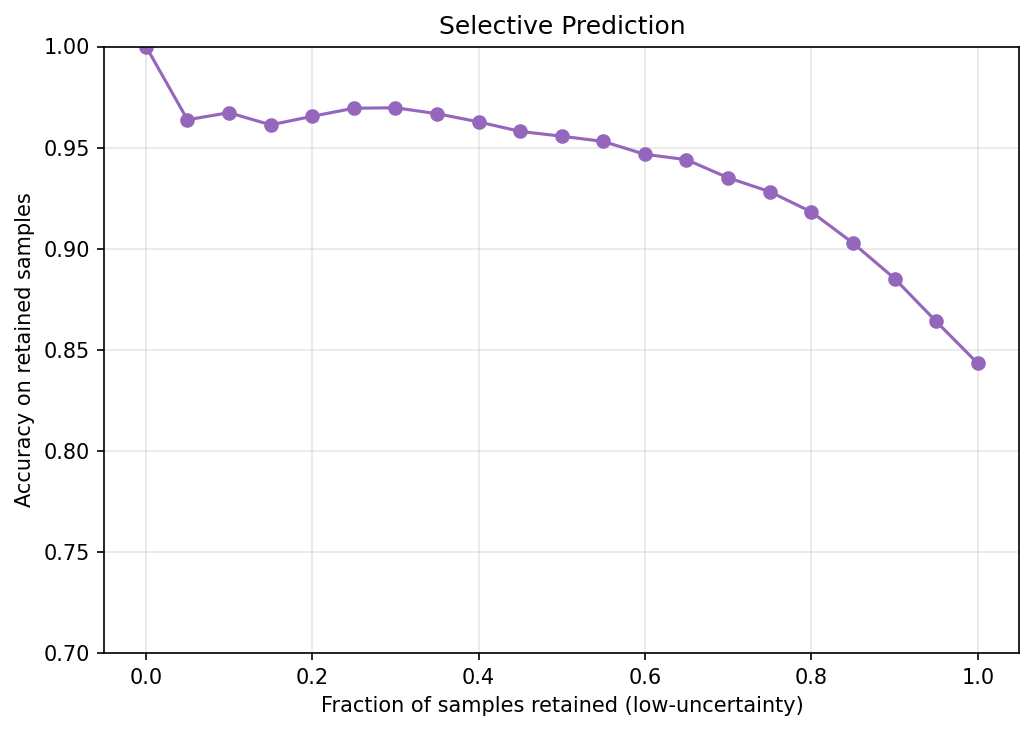
\includegraphics[width=\columnwidth]{figures/selective_prediction.png}
\caption{Selective prediction: by referring the highest-entropy samples to a human reviewer, accuracy on the retained low-uncertainty samples increases monotonically. A clinically deployable safety mechanism.}
\label{fig:selective}
\end{figure}

\subsection{MC Dropout Uncertainty}
The MC Dropout extension on the full test set ($N{=}2750$, $T{=}20$ passes per image) yields the following key findings (Table~\ref{tab:perclass}, last two rows; Fig.~\ref{fig:uncertainty}; Fig.~\ref{fig:selective}):
\begin{itemize}
    \item \textbf{Uncertainty separates correct from wrong predictions.} Mean predictive entropy is 0.37 on correct predictions vs.\ 0.77 on wrong predictions --- a $2.07\times$ separation.
    \item \textbf{Uncertainty correlates with class difficulty.} The model's entropy is lowest on the easy Grade 0 ($\overline{H}{=}0.32$) and highest on Grades 2--4 ($\overline{H}\geq 0.76$), matching the failure-mode breakdown.
    \item \textbf{Selective prediction is effective.} When retaining only low-uncertainty samples, accuracy on the retained cohort increases monotonically, supporting deployment as a triage system that defers ambiguous cases to a specialist.
\end{itemize}

\subsection{Limitation: Mutual Information Collapse}
A negative but informative finding: the \emph{mutual information} $I$ between MC samples is approximately zero across all test samples. This means the $T{=}20$ stochastic passes produced near-identical outputs, and the predictive entropy is dominated by the aleatoric component (i.e., softmax sharpness from the deterministic backbone). The cause is structural: dropout is only present in the DRSA transformer block (a single layer with $p{=}0.1$), while the ResNet-50 backbone is fully deterministic. Consequently, the Bayesian approximation collapses and what we measure as ``uncertainty'' is best interpreted as predictive entropy --- still highly useful for selective prediction, as we have shown, but not a faithful estimate of epistemic uncertainty.

This finding motivates future work to either (a) increase dropout rate and add dropout to the backbone before retraining, or (b) replace dropout with proper Bayesian layers (e.g., Bayes by Backprop \cite{blundell2015bbb} or variational dropout) for genuine epistemic estimates.

% ==========================================================================
\section{Conclusions}
We extended a self-explainable hybrid CNN--Transformer for DR detection with a Bayesian uncertainty mechanism via MC Dropout, requiring no retraining. The base model achieves kappa $0.811$ on the Kaggle 2015 DR test set, exceeding prior work. The added uncertainty estimates separate correct from incorrect predictions by a $2.07\times$ entropy gap and support a deployable selective-prediction strategy. We also identified that pure MC Dropout collapses to deterministic inference in this architecture, motivating richer Bayesian designs as future work. Together, interpretable evidence maps plus calibrated uncertainty form a clinically meaningful combination: the model explains \emph{where} it is looking and signals \emph{when it does not know}.

% ==========================================================================
\begin{thebibliography}{99}

\bibitem{flaxman2017global}
S.\ R.\ Flaxman \emph{et al.}, ``Global causes of blindness and distance vision impairment 1990--2020,'' \emph{The Lancet Global Health}, vol.\ 5, no.\ 12, pp.\ e1221--e1234, 2017.

\bibitem{selvaraju2017gradcam}
R.\ R.\ Selvaraju \emph{et al.}, ``Grad-CAM: Visual explanations from deep networks via gradient-based localization,'' in \emph{Proc.\ IEEE Int.\ Conf.\ Computer Vision (ICCV)}, 2017, pp.\ 618--626.

\bibitem{ilyas2024hybrid}
T.\ Ilyas \emph{et al.}, ``A hybrid CNN--Transformer feature pyramid network for medical image analysis,'' \emph{Medical Image Analysis}, vol.\ 91, p.\ 103011, 2024.

\bibitem{dosovitskiy2020vit}
A.\ Dosovitskiy \emph{et al.}, ``An image is worth 16$\times$16 words: Transformers for image recognition at scale,'' in \emph{Proc.\ Int.\ Conf.\ Learning Representations (ICLR)}, 2021.

\bibitem{djoumessi2025hybrid}
K.\ Djoumessi, S.\ O.\ Mensah, and P.\ Berens, ``A hybrid fully convolutional CNN--Transformer model for inherently interpretable disease detection from retinal fundus images,'' in \emph{8th Int.\ Workshop on Interpretability of Machine Intelligence in Medical Image Computing (IMIMIC) at MICCAI}, 2025. arXiv:2504.08481.

\bibitem{gal2016dropout}
Y.\ Gal and Z.\ Ghahramani, ``Dropout as a Bayesian approximation: Representing model uncertainty in deep learning,'' in \emph{Proc.\ Int.\ Conf.\ Machine Learning (ICML)}, 2016, pp.\ 1050--1059.

\bibitem{he2016deep}
K.\ He, X.\ Zhang, S.\ Ren, and J.\ Sun, ``Deep residual learning for image recognition,'' in \emph{Proc.\ IEEE Conf.\ Computer Vision and Pattern Recognition (CVPR)}, 2016, pp.\ 770--778.

\bibitem{kaggleDR2015}
Kaggle, ``Diabetic Retinopathy Detection,'' Kaggle Competition, 2015. \url{https://www.kaggle.com/c/diabetic-retinopathy-detection}.

\bibitem{blundell2015bbb}
C.\ Blundell, J.\ Cornebise, K.\ Kavukcuoglu, and D.\ Wierstra, ``Weight uncertainty in neural networks,'' in \emph{Proc.\ Int.\ Conf.\ Machine Learning (ICML)}, 2015, pp.\ 1613--1622.

\bibitem{brendel2018bagnet}
W.\ Brendel and M.\ Bethge, ``Approximating CNNs with bag-of-local-features models works surprisingly well on ImageNet,'' in \emph{Proc.\ Int.\ Conf.\ Learning Representations (ICLR)}, 2019.

\end{thebibliography}

\end{document}
